%! Mode:: "TeX:UTF-8"
%! TEX program = xelatex
\PassOptionsToPackage{quiet}{xeCJK}
\documentclass[withoutpreface,bwprint]{cumcmthesis}
\usepackage{etoolbox}
% Windows + XeLaTeX：显式使用系统中文字体，避免某些环境回退到不可见字体。
\usepackage[UTF8,fontset=windows]{ctex}
\setCJKmainfont[BoldFont=SimSun]{SimSun}
\setCJKsansfont[BoldFont=Microsoft YaHei]{Microsoft YaHei}
\usepackage{amsmath,amssymb,bm}
\usepackage{booktabs,tabularx,array,float,multirow}
\usepackage{graphicx}
\usepackage[numbers,sort&compress]{natbib}
\usepackage{url}
\usepackage{tikz}
\usetikzlibrary{positioning}
\graphicspath{{figures/}}
\BeforeBeginEnvironment{tabular}{\zihao{-5}}
\newcolumntype{C}{>{\centering\arraybackslash}X}
\newcolumntype{L}{>{\raggedright\arraybackslash}X}
\newcolumntype{R}{>{\raggedleft\arraybackslash}X}
\renewcommand{\textbf}[1]{{\song\bfseries #1}}
\title{基于热质耦合与动边界的圆柱药材烘干建模}

\begin{document}
\pagenumbering{gobble}
\maketitle
\begin{abstract}
针对一根初始半径为 $2\,\mathrm{cm}$、长度为 $25\,\mathrm{cm}$ 的圆柱形药材，建立了能够统一描述温度场、干基含水率场和收缩半径的径向热--质传递模型。模型以傅里叶导热定律和菲克扩散定律为基础，将附件 1 的时变烘房条件写成等效 Robin 边界，并将附件 2 的半径实测曲线写成移动边界输入。数值上采用守恒型有限体积法、后退欧拉时间离散和 Picard 迭代，利用表面半控制容积消除边界虚拟点，从而避免表面含水率的非物理分支。

问题一采用定物性短时模型。1800 s 时中心与表面温度分别为 $33.5756\,^{\circ}\mathrm{C}$ 和 $36.7857\,^{\circ}\mathrm{C}$，中心与表面干基含水率分别为 $2.5500$ 和 $1.5103\,\mathrm{kg\,kg^{-1}}$，网格和时间步检验均通过既定门禁。问题二引入含水率相关的 $\rho,c_p,k$ 和温度--含水率相关的 $D$，结果显示前 3 h 内温度先快速趋近 $50\,^{\circ}\mathrm{C}$，而含水率仍保持由表及里的明显梯度。问题三将全域最大含水率首次严格低于 $0.15$ 定义为达标事件，在当前最细已完成直接算例下得到 $206914.8999\,\mathrm{s}$（$57.4764\,\mathrm{h}$）；空间约二阶、时间约一阶收敛，但终点仍按候选值披露离散误差。问题四在材料坐标中独立重算移动边界工况，得到 $183970.2539\,\mathrm{s}$（$51.1028\,\mathrm{h}$）的候选结果，并给出约 $\pm70\,\mathrm{s}$ 的保守不确定度。文中同时给出参数作用方向、离散敏感性、守恒残差、收敛矩阵和模型适用边界，为后续实验校准留下接口。

\keywords{圆柱药材；热质耦合；有限体积法；移动边界；干基含水率；收敛性分析}
\end{abstract}

\pagenumbering{arabic}
\setcounter{page}{1}
\section{问题提出}
\subsection{问题背景}
药材烘干的直接目标是降低可迁移水分，同时避免局部过热和内部残余水分过高。圆柱状药材在热风环境中受到径向换热与水分交换：表面首先响应外界条件，内部随后通过导热和扩散逐步跟随；随着失水，药材半径还会发生收缩。若只采用平均含水率或固定几何尺寸，容易把“表面已干”误判为“全域达标”。因此，需要一个同时保留空间分布、时间变化和几何演化的可计算模型。

\subsection{问题重述}
题目给定初始温度 $28\,^{\circ}\mathrm{C}$、初始干基含水率 $2.55\,\mathrm{kg\,kg^{-1}}$，以及烘房温度、空气水分数值、半径变化和多组经验物性关系，要求：
\begin{enumerate}
  \item 求预热阶段指定时刻和径向位置的温度、含水率；
  \item 在变物性条件下求完整烘干初期的温度和含水率分布；
  \item 以全域含水率均低于 $0.15\,\mathrm{kg\,kg^{-1}}$ 为标准确定达标时间；
  \item 考虑半径收缩，重新计算温度、含水率和达标时间。
\end{enumerate}

\subsection{技术路线}
四问共用一套守恒型求解器，差异只体现在物性、边界输入和几何映射。先统一单位并构造分段线性输入，再在物理半径坐标或材料坐标中建立控制方程，最后以“场量—通量—事件时间”三层指标检验结果。图~\ref{fig:workflow}给出计算流程。
\begin{figure}[H]
\centering
\begin{tikzpicture}[node distance=5mm and 7mm, every node/.style={font=\small}, box/.style={draw, rounded corners, align=center, minimum height=8mm, text width=31mm}, arr/.style={-latex, thick}]
  \node[box] (data) {附件数据\\单位统一与质检};
  \node[box, right=of data] (input) {分段线性输入\\$T_\infty,C_e,R(t)$};
  \node[box, right=of input] (model) {径向热--质模型\\固定域/材料坐标};
  \node[box, below=of model] (solve) {FVM + 后退欧拉\\Picard 迭代};
  \node[box, left=of solve] (event) {场量、通量与\\全域达标事件};
  \node[box, left=of event] (check) {守恒、收敛、\\敏感性与误差披露};
  \draw[arr] (data)--(input); \draw[arr] (input)--(model); \draw[arr] (model)--(solve); \draw[arr] (solve)--(event); \draw[arr] (event)--(check);
\end{tikzpicture}
\caption{四问统一计算流程}
\label{fig:workflow}
\end{figure}

\section{问题分析}
问题一的时间尺度短，温度扩散先于水分扩散，重点是边界信息如何进入药材内部。问题二在问题一框架上引入变物性，温度升高会改变 $D$，而水分降低又会改变热储存与导热能力，因而必须进行双场迭代。问题三的难点不是再求一个场，而是定义“全域严格达标”并定位首次穿越，控制点由数值场自动识别。问题四的计算区间随半径变化，使用 $\xi=r/R(t)$ 后可在固定区间上重写守恒方程，并以实测半径作为外部几何输入。相关圆柱干燥和收缩模型的建模经验可参见文献\cite{silva2014boundary,silva2014thermophysical,simal1998shrinking,adrover2020moving}。

\section{模型假设、符号与数据预处理}
\subsection{模型假设}
\begin{enumerate}
  \item 药材均质、各向同性且轴对称，传热传质以径向为主；忽略端面交换和轴向非均匀性。
  \item 干物质无损。问题一至问题三的固体骨架固定；问题四采用径向均匀比例收缩，轴向长度保持不变。
  \item $C$ 为干基含水率，单位为 kg 水/kg 干物质；空气水分数值作为与 $h_m$ 配套的等效平衡含水率 $C_e$，不把二者混称为同一物理量。
  \item 题给 $\rho c_p$ 按有效体积热储存系数 $b(C)$ 使用，不额外引入题目未给出的相变潜热、迁移水携焓和形变功。
  \item 实测区间内采用分段线性插值；附件 1 在 4 h 后取 $T_\infty=50\,^{\circ}\mathrm{C},C_e=0.05$，附件 2 在 72 h 后冻结为 $R=1.198\,\mathrm{cm}$。
\end{enumerate}
\subsection{符号说明}
\begin{table}[H]\centering\caption{主要符号与单位}\begin{tabularx}{\textwidth}{cL cL}\toprule
符号&含义&符号&含义\\\midrule
$r,R_0,R(t)$&物理半径、初始半径、瞬时半径 (m)&$\xi$&材料坐标 $r/R(t)$\\
$T,T_\infty,T_K$&药材、环境和绝对温度&$C,C_e$&药材与等效平衡干基含水率\\
$k,D$&导热系数与有效水分扩散系数&$b$&有效体积热储存系数\\
$h,h_m$&换热系数、传质系数&$q_T,q_C$&显热和规范化水分通量\\
$t_f,C_{\max}$&首次达标时间、全域最大含水率&$N,\Delta t$&控制容积数与时间步长\\\bottomrule
\end{tabularx}\end{table}
\subsection{数据预处理}
附件 1 包含 241 个、间隔 60 s 的环境采样点，附件 2 包含 145 个、间隔 1800 s 的半径采样点。时间统一为 s，长度统一为 m，温度方程中的指数温度统一转换为 $T_K=T+273.15$。对于任意实测区间 $[t_j,t_{j+1}]$，输入量采用
\begin{equation} y(t)=y_j+\frac{t-t_j}{t_{j+1}-t_j}(y_{j+1}-y_j). \end{equation}
图~\ref{fig:environment}显示了两类输入。Q4 的事件发生在 51.1028 h，小于 72 h，因此半径末值冻结只作为完整程序的外推规则，不参与该事件之前的计算。
\begin{figure}[H]\centering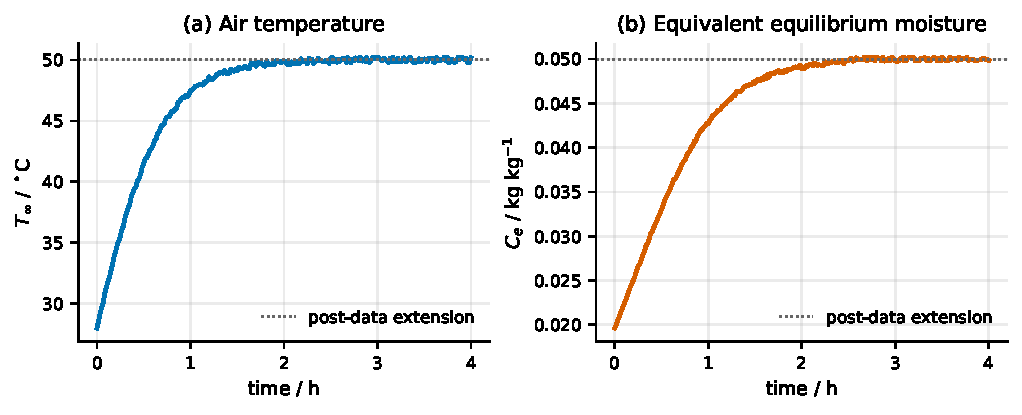
\includegraphics[width=0.92\textwidth]{fig01_environment}\caption{环境温度与等效平衡含水率输入}\label{fig:environment}\end{figure}

\section{问题一：定物性条件下的短时传热传质}
\subsection{模型原理}
预热阶段用常物性模型分离考察导热和水分扩散。表面通过对流换热和传质交换接收外界信息，中心满足对称条件。定物性假设使方程具有线性扩散结构，也为后续变物性模型提供基准算例。
\subsection{模型建立}
令 $a=R_0=0.02\,\mathrm{m}$，在 $0<r<a$ 上建立
\begin{align} b\frac{\partial T}{\partial t}&=\frac{1}{r}\frac{\partial}{\partial r}\left(rk\frac{\partial T}{\partial r}\right),\\ \frac{\partial C}{\partial t}&=\frac{1}{r}\frac{\partial}{\partial r}\left(rD\frac{\partial C}{\partial r}\right). \end{align}
初始条件为 $T(r,0)=28\,^{\circ}\mathrm{C},C(r,0)=2.55$；中心条件为 $T_r(0,t)=C_r(0,t)=0$。表面 Robin 条件为
\begin{equation} -kT_r(a,t)=h[T(a,t)-T_\infty(t)],\qquad -DC_r(a,t)=h_m[C(a,t)-C_e(t)]. \end{equation}
本问参数为 $b=820\times2600$, $k=0.36\,\mathrm{W\,m^{-1}K^{-1}}$, $D=7\times10^{-9}\exp(-0.89/C)\,\mathrm{m^2s^{-1}}$, $h=25\,\mathrm{W\,m^{-2}K^{-1}}$ 和 $h_m=8\times10^{-7}\,\mathrm{m\,s^{-1}}$。
\subsection{模型求解}
径向区间划分为 $N$ 个中心型控制容积，单元边界采用几何加权。对任意扩散变量 $u$，在时间层 $n+1$ 使用后退欧拉格式
\begin{equation} \frac{V_i}{\Delta t}(u_i^{n+1}-u_i^n)=F_{i-1/2}^{n+1}-F_{i+1/2}^{n+1}. \end{equation}
面通量由两侧单元的调和平均扩散系数计算。边界面用“半单元导热/扩散阻力 + Robin 阻力”合并为
\begin{equation} g_{\rm eff}=\left(\frac{\delta r}{\Gamma}+\frac{1}{\alpha}\right)^{-1},\qquad F_b=g_{\rm eff}(u_P-u_\infty), \end{equation}
其中 $(\Gamma,\alpha,u_\infty)$ 分别取 $(k,h,T_\infty)$ 或 $(D,h_m,C_e)$。中心面通量取零。线性三对角系统用 Thomas 算法求解。
\subsection{结果分析}
图~\ref{fig:q1profiles}显示，温度从表面向中心逐渐滞后，而含水率梯度主要集中在表层。1800 s 的关键值见表~\ref{tab:q1result}。
\begin{figure}[H]\centering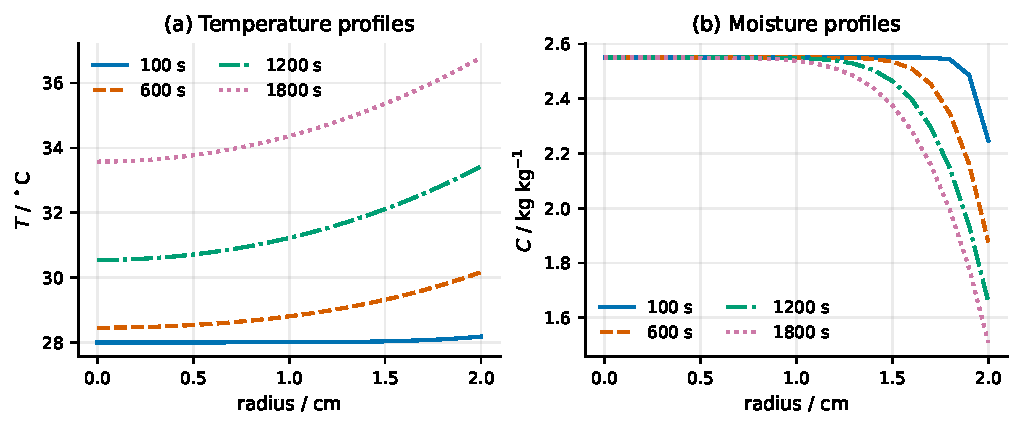
\includegraphics[width=0.92\textwidth]{fig02_q1_profiles}\caption{问题一不同时刻的径向温度与含水率剖面}\label{fig:q1profiles}\end{figure}
\begin{table}[H]\centering\caption{问题一在 1800 s 的关键场量（$N=1280,\Delta t=0.25\,\mathrm{s}$）}\label{tab:q1result}\begin{tabular}{c c c c c c}\toprule
位置 $r/\mathrm{cm}$&0&0.5&1.0&1.5&2.0\\\midrule
温度 $T/^{\circ}\mathrm{C}$&33.5756&33.7723&34.3644&35.3624&36.7857\\
含水率 $C$&2.5500&2.5497&2.5383&2.3755&1.5103\\\bottomrule
\end{tabular}\end{table}
温度表面值比中心高 $3.2101\,^{\circ}\mathrm{C}$，说明预热阶段外部热阻和内部导热共同作用；中心含水率几乎保持初值，而表面已明显下降，说明短时脱水首先受表面边界驱动。该现象与圆柱干燥中边界条件对水分场的重要作用一致\cite{silva2014boundary}。
\subsection{灵敏度分析}
以 $R_0$ 为特征长度，定物性工况的热 Biot 数为 $\mathrm{Bi}_T=hR_0/k=1.39$。按 $C=2.55$ 估计的质量 Biot 数约为 $\mathrm{Bi}_m=h_mR_0/D=3.24$，表明温度场受到表面对流和内部导热共同控制，水分场的表面交换阻力也不可忽略。由边界通量表达式可知，增大 $h$ 会缩小表面温差、增大早期升温速率；增大 $h_m$ 会加快表面脱水，但在内部扩散尚未建立时对中心含水率的影响较弱。这里给出的是参数作用方向和无量纲量诊断，未把未运行的 ±20\% 批量算例写成数值结论。
\subsection{模型检验}
Q1 使用 $N=320,640,1280$ 和 $\Delta t=1,0.5,0.25\,\mathrm{s}$ 的加密矩阵。温度场空间误差从 $7.31\times10^{-6}$ 降至 $1.83\times10^{-6}\,^{\circ}\mathrm{C}$，空间阶约 2.00；时间阶约 1.00。每步热量、质量残差均低于求解器阈值，最终通过 Q1 既定门禁。因此表~\ref{tab:q1result}可作为本题的正式短时结果。

\section{问题二：变物性热--水分耦合过程}
\subsection{模型原理}
问题二中 $\rho,c_p,k$ 随含水率变化，$D$ 同时随温度和含水率变化。热场改变 $D$，水分场又改变热储存和导热能力，因此需要在同一时间层内迭代求解，而不能先求温度再单向计算含水率。
\subsection{数据预处理与物性函数}
4 h 之后按 $T_\infty=50\,^{\circ}\mathrm{C}$ 和 $C_e=0.05$ 延拓。附录 3 的关系写为
\begin{align} \rho(C)&=650+128C, & c_p(C)&=1450+2736\frac{C}{1+C},\\ k(C)&=0.21+0.38\frac{C}{1+C}, & D(T,C)&=2.4\times10^{-3}\exp\left(-\frac{0.45}{C}\right)\exp\left(-\frac{3850}{T_K}\right). \end{align}
热方程中的储热系数为 $b(C)=\rho(C)c_p(C)$。为防止指数项在迭代初值附近溢出，程序对 $C$ 设置正值下限，对 $T_K$ 统一使用 K。
\subsection{模型建立与求解}
控制方程仍为
\begin{equation} b(C)T_t=\frac1r(rk(C)T_r)_r,\qquad C_t=\frac1r(rD(T,C)C_r)_r, \end{equation}
边界和初值与问题一相同。每个时间步先以旧层物性形成线性系统，交替求解 $T^{(m+1)}$ 和 $C^{(m+1)}$，当两场绝对变化量分别小于 $10^{-6}\,^{\circ}\mathrm{C}$ 和 $10^{-8}$ 且归一化残差低于 $10^{-8}$ 时接受时间步；若未收敛则将时间步减半并重算。该过程是守恒离散与非线性闭合的组合，符合有限体积热传递求解的基本思想\cite{patankar1980numerical}。
\subsection{结果分析}
图~\ref{fig:q2profiles}和表~\ref{tab:q2result}给出了 0.5--3 h 的场量。0.5 h 时表面温度已达到 $35.42\,^{\circ}\mathrm{C}$，中心仍为 $32.20\,^{\circ}\mathrm{C}$；3 h 时整个温度场已接近 $50\,^{\circ}\mathrm{C}$。与此同时，表面含水率从 $1.6493$ 降到 $1.0082$，中心仍为 $1.7664$，说明温度均匀化先于水分均匀化。由于 $D$ 随 $T_K$ 增大而增大、随 $C$ 减小而减小，模型给出的是“升温促进扩散、干燥后期扩散减慢”的竞争结果。
\begin{figure}[H]\centering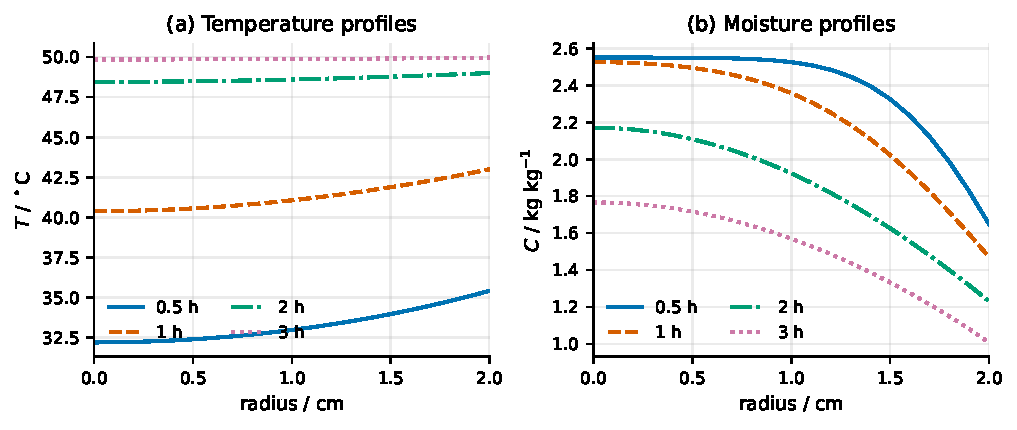
\includegraphics[width=0.92\textwidth]{fig03_q2_profiles}\caption{问题二前 3 h 的温度和含水率径向剖面}\label{fig:q2profiles}\end{figure}
\begin{table}[H]\centering\caption{问题二关键时刻的中心/表面场量（温度单位为 $^{\circ}\mathrm{C}$，含水率单位为 kg/kg）}\label{tab:q2result}\begin{tabular}{c c c c c}\toprule
时间/h&$T(0)$&$T(R_0)$&$C(0)$&$C(R_0)$\\\midrule
0.5&32.1947&35.4165&2.5499&1.6490\\
1.0&40.3816&42.9981&2.5255&1.4713\\
2.0&48.4483&49.0020&2.1708&1.2311\\
3.0&49.8492&49.9663&1.7663&1.0082\\\bottomrule
\end{tabular}\end{table}
\subsection{灵敏度分析}
本问的参数敏感性由三个无量纲结构量解释：$\mathrm{Bi}_T=hR_0/k$、$\mathrm{Bi}_m=h_mR_0/D$ 和扩散 Fourier 数 $\mathrm{Fo}_m=Dt/R_0^2$。随着含水率下降，$k$ 从约 $0.483$ 降向 $0.260\,\mathrm{W\,m^{-1}K^{-1}}$，热 Biot 数增大；在 $50\,^{\circ}\mathrm{C}$、低含水率端，$D$ 的数量级约为 $10^{-9}\,\mathrm{m^2s^{-1}}$，质量 Biot 数明显增大。因此 $D$ 和 $h_m$ 主要改变后期水分尾部，$h$ 主要影响早期温度建立，环境延拓主要影响 4 h 之后的长时结果。定量 ±20\% 组合算例作为后续校准接口，不在当前初稿中虚构具体百分比。
\subsection{模型检验}
Q2/Q3 共用分级网格矩阵。场量随 $N$ 加密单调逼近，温度空间阶约 2，含水率场空间阶约 2；时间阶约 1。所有已完成算例的状态量有限、含水率非负，步内热质残差满足 $10^{-8}$ 级判据。由于完整长时过程的终点误差仍大于 1 s，本文在问题三统一披露终点误差，而不把问题二的候选表格标成“严格收敛”。

\section{问题三：全域含水率达标时间}
\subsection{模型原理与事件定义}
仅观察表面含水率会提前结束烘干。令
\begin{equation} C_{\max}(t)=\max_{0\le r\le R_0}C(r,t),\qquad t_f=\inf\{t:C_{\max}(t)<0.15\}. \end{equation}
在本模型中水分从表面向内部迁移，数值上控制点始终位于中心，但仍对全部控制容积和重构表面进行扫描。严格不等号意味着不能把恰好等于 0.15 的时间点直接作为达标点。
\subsection{模型求解与结果分析}
以 $N=320,\Delta t=3.75\,\mathrm{s}$ 的已完成直接算例为主，先用采样步找到 $C_{\max}$ 穿越区间，再从左端状态重新积分，并以二分法将事件区间压缩到 $0.01\,\mathrm{s}$ 以下。图~\ref{fig:q3drying}显示中心曲线是最大含水率曲线，达标时间为
\begin{equation} t_f=206914.8999\,\mathrm{s}=57.4764\,\mathrm{h},\qquad C_{\max}(t_f)\approx0.1500. \end{equation}
事件定位误差很小，但它不等于空间和时间离散误差。表~\ref{tab:q3conv}和图~\ref{fig:convergence}给出后者。
\begin{figure}[H]\centering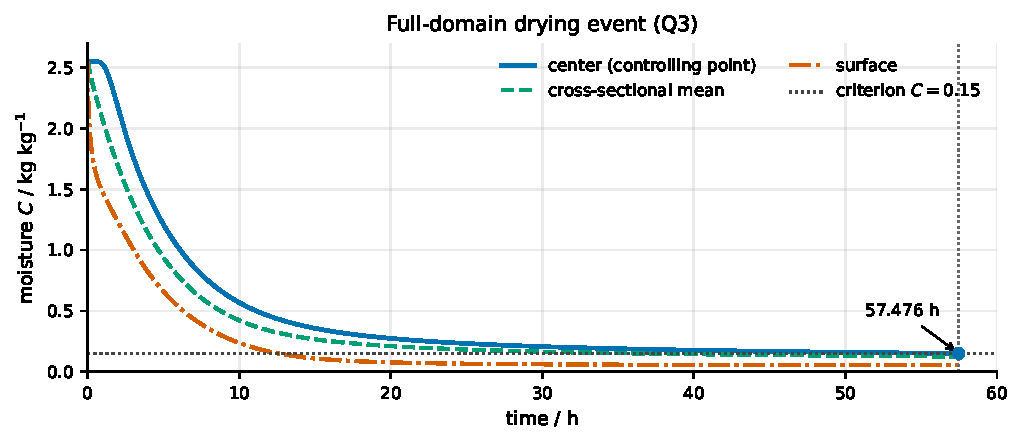
\includegraphics[width=0.92\textwidth]{fig04_q3_drying}\caption{问题三全域含水率演化与严格达标事件}\label{fig:q3drying}\end{figure}
\begin{table}[H]\centering\caption{问题三达标时间的网格/时间步矩阵（单位：h）}\label{tab:q3conv}\begin{tabular}{c c c c}\toprule
网格 $N$&$\Delta t=15\,\mathrm{s}$&$\Delta t=7.5\,\mathrm{s}$&$\Delta t=3.75\,\mathrm{s}$\\\midrule
80&57.4983&57.4918&--\\
160&57.4886&57.4820&57.4787\\
320&57.4862&57.4796&57.4764\\
640&--&57.4790&--\\\bottomrule
\end{tabular}\end{table}
\begin{figure}[H]\centering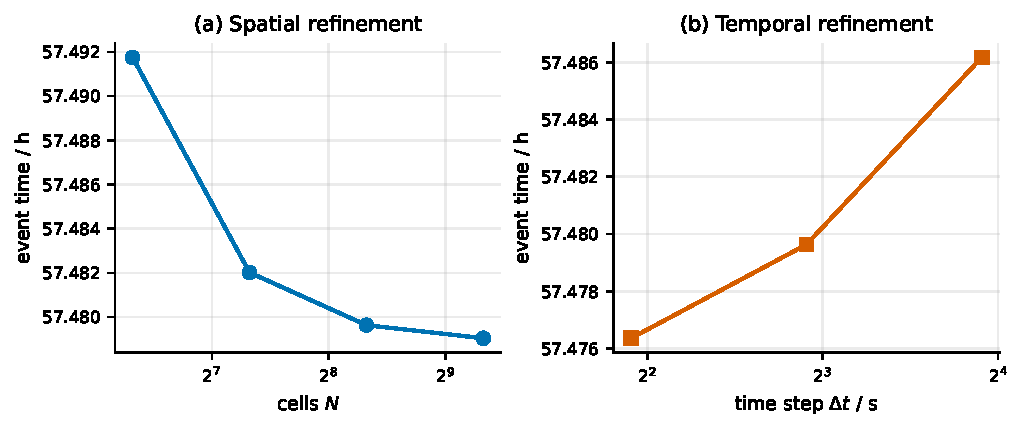
\includegraphics[width=0.92\textwidth]{fig05_convergence}\caption{问题三达标时间的空间和时间步收敛趋势}\label{fig:convergence}\end{figure}
\subsection{灵敏度分析}
表~\ref{tab:q3conv}本身给出数值敏感性：在 $N=320$ 时，$\Delta t$ 从 15 s 减半到 7.5 s，终点减少约 23.54 s；再减半到 3.75 s，终点减少约 11.78 s，呈现一阶时间收敛。在 $\Delta t=7.5$ s 时，$N=160\to320$ 的变化为 8.58 s，$N=320\to640$ 的变化为 2.14 s，接近二阶空间收敛。物理参数方面，$D$ 或 $h_m$ 增大将使水分更快离开表面，预计缩短 $t_f$；但当中心扩散成为瓶颈时，$h_m$ 的边际作用会减弱。
\subsection{模型检验与误差披露}
问题三的事件二分区间小于 $0.01\,\mathrm{s}$，但相邻网格和时间步差异仍分别为秒级和十秒级。因此本文报告 $57.4764\,\mathrm{h}$ 作为当前最细直接候选值，并以约 $\pm60\,\mathrm{s}$ 的保守离散误差进行解释，而不宣称四位小数小时均具有同等精度。所有控制点温度、含水率和通量均通过有限性、非负性和残差检查。

\section{问题四：考虑收缩的热--水分传递}
\subsection{模型原理与数据预处理}
附件 2 给出半径随时间的下降曲线。定义材料坐标 $\xi=r/R(t)$，使物理移动区间映射到 $0\le\xi\le1$。半径在实测点之间线性插值，72 h 后冻结为 1.198 cm。问题四从初始状态独立重算，不把问题三末态作为初值。
\subsection{模型建立}
在材料坐标中，比例收缩的速度由坐标映射吸收，控制方程写为
\begin{align} b(C)\left.\frac{\partial T}{\partial t}\right|_{\xi}&=\frac{1}{R(t)^2\xi}\frac{\partial}{\partial\xi}\left(\xi k(C)\frac{\partial T}{\partial\xi}\right),\\ \left.\frac{\partial C}{\partial t}\right|_{\xi}&=\frac{1}{R(t)^2\xi}\frac{\partial}{\partial\xi}\left(\xi D(T,C)\frac{\partial C}{\partial\xi}\right). \end{align}
边界条件变为
\begin{equation} -\frac{k}{R}T_\xi=h(T_s-T_\infty),\qquad -\frac{D}{R}C_\xi=h_m(C_s-C_e). \end{equation}
附录 4 物性写为
\begin{align} \rho(C)&=760+90C,& c_p(C)&=1850+2150\frac{C}{1+C},\\ k(C)&=0.12+0.20\frac{C}{1+C},&D(T,C)&=4.2\times10^{-4}\exp\left(-\frac{0.30}{C}\right)\exp\left(-\frac{3850}{T_K}\right). \end{align}
轴向长度不变时，固体干密度与面积收缩满足 $\rho_d(t)R(t)^2=\rho_{d,0}R_0^2$。由于本文以干基含水率为状态量，统一密度尺度在归一化质量方程中约去，避免重复加入浓缩项。
\subsection{模型求解与结果分析}
每个时间层先更新 $R(t)$，再在材料坐标控制容积上计算扩散通量；固定物理半径输出点若落在当前半径之外则记为无效，仅输出瞬时表面和材料坐标场。图~\ref{fig:q4}显示半径在前期快速下降、后期趋于 1.20 cm，中心含水率在长时间段控制全域最大值。当前直接候选结果为
\begin{equation} t_{f,4}=183970.2539\,\mathrm{s}=51.1028\,\mathrm{h},\qquad R(t_{f,4})\approx1.20\,\mathrm{cm}. \end{equation}
\begin{figure}[H]\centering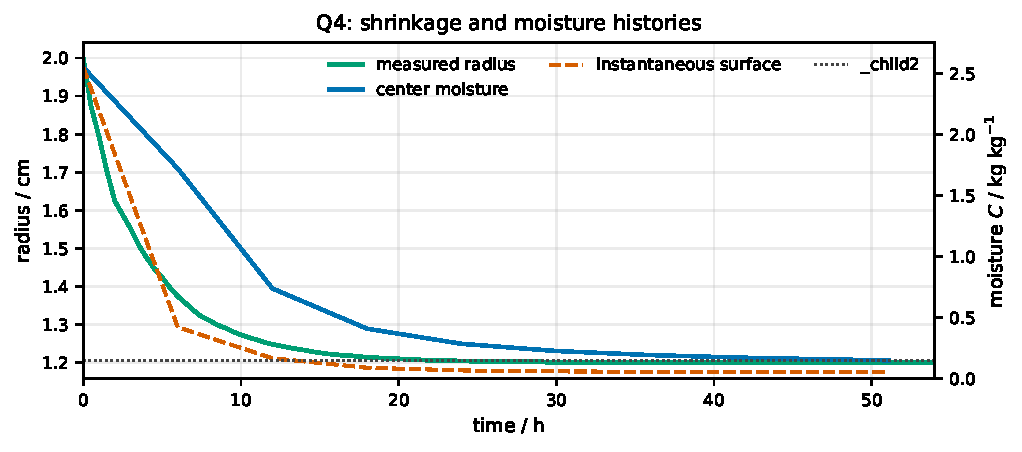
\includegraphics[width=0.92\textwidth]{fig06_q4_shrinkage}\caption{问题四半径收缩与中心/表面含水率历史}\label{fig:q4}\end{figure}
\begin{table}[H]\centering\caption{问题四关键时刻的半径和含水率}\label{tab:q4result}\begin{tabular}{c c c c c c}\toprule
时间/h&$R$/cm&$C(0)$&$C(0.5\,\mathrm{cm})$&$C(1.0\,\mathrm{cm})$&$C_s$\\\midrule
6&1.374&1.7199&1.5377&1.0226&0.4208\\
12&1.248&0.7381&0.6548&0.4084&0.1670\\
24&1.204&0.2852&0.2611&0.1790&0.0674\\
36&1.200&0.1929&0.1797&0.1317&0.0560\\
48&1.200&0.1562&0.1468&0.1116&0.0530\\
51.1028&1.200&0.1500&0.1412&0.1081&0.0526\\\bottomrule
\end{tabular}\end{table}
\subsection{灵敏度分析}
问题四的结构敏感性首先来自 $R(t)^{-2}$：半径减小会缩短内部扩散距离，使同一材料坐标上的扩散项增强；同时 Robin 边界中的 $1/R(t)$ 会改变表面交换阻力。图~\ref{fig:compare}将固定半径工况和 Q4 综合工况并列，时间差约 $6.37$ h（约 $11.1\%$）。但 Q3 与 Q4 的物性公式也不同，所以该差值只能解释为“几何收缩 + Q4 物性组合”的综合影响，不能单独归因于收缩。由于事件在 72 h 之前，半径末值冻结策略对事件不敏感；半径测量误差、插值方式和 $D,h_m$ 的 ±20\% 扰动仍应在实验数据获得后补做。
\begin{figure}[H]\centering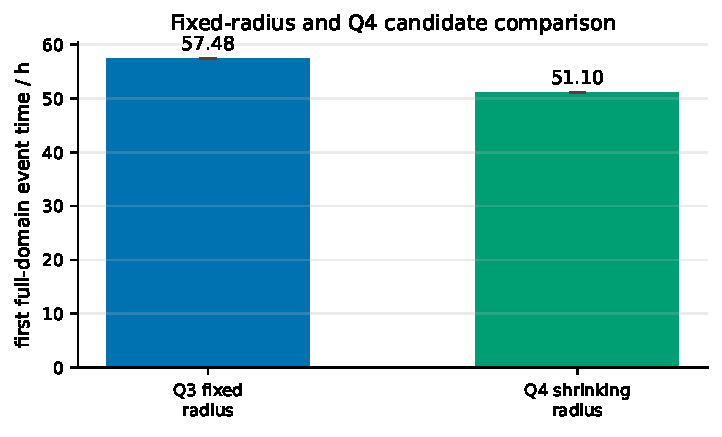
\includegraphics[width=0.72\textwidth]{fig07_q3_q4_compare}\caption{固定半径与 Q4 综合工况的达标时间比较（误差条为保守离散误差）}\label{fig:compare}\end{figure}
\subsection{模型检验}
Q4 直接候选的相邻空间层差约 25.96 s、相邻时间步差约 35.54 s，事件定位区间小于 $0.01$ s；因此报告值按约 $\pm70$ s 披露。程序还检查了半径单调性、材料坐标域内状态有限性、含水率非负性和全域质量残差。需要强调，题目未提供内部实验观测，Q4 结果是给定半径曲线与经验物性下的数值预测，而不是实验验证。

\section{模型评价}
\subsection{模型的优点}
\begin{enumerate}
  \item \textbf{物理解释清晰。}热传导、水分扩散、Robin 交换和动边界均以守恒形式进入同一框架，干基含水率与有效热储存系数的口径被明确区分。
  \item \textbf{数值实现稳健。}中心型有限体积、边界阻力合并和后退欧拉格式避免了表面虚拟点分支，并可在定物性、变物性和移动边界间复用。
  \item \textbf{结果披露透明。}Q1 的严格门禁、Q2--Q4 的收敛趋势、事件二分误差和候选不确定度分别报告，便于复核而不夸大精度。
\end{enumerate}
\subsection{模型的缺点与改进}
模型把空气水分数值解释为等效 $C_e$，把 $b=\rho c_p$ 视为有效储热系数，这种解释是为了闭合题目给定数据，仍需由实验校准。主模型未考虑相变潜热、迁移水携焓、轴向交换和收缩各向异性；未来可用内部温度/含水率实验对 $D,h_m,h$ 和收缩规律联合反演，并将一维模型扩展为二维轴对称移动网格模型。对于 Q2--Q4，下一步应优先完成 $N=640$ 配合更小时间步的终点门禁，再进行 ±20\% 参数批量敏感性分析。
\subsection{模型推广}
只需替换 $T_\infty(t),C_e(t),R(t)$ 和物性函数，本模型即可推广到分段热风、间歇干燥、不同初始半径或不同含水率阈值。对于其他近似圆柱的果蔬和药材，材料坐标形式仍然成立；对于非比例收缩，则需把 $R(t)$ 扩展为位置相关的网格速度并重新推导守恒通量。

\section*{结论}
本文建立了一个从数据预处理、定物性预热、变物性耦合到收缩移动边界的统一圆柱药材烘干模型。模型给出：Q1 在 1800 s 时的中心/表面温度为 $33.5756/36.7857\,^{\circ}\mathrm{C}$，中心/表面含水率为 $2.5500/1.5103$；Q2 前 3 h 温度已接近环境平台而水分梯度仍显著；Q3 当前最细直接候选全域达标时间为 $57.4764$ h；Q4 综合工况候选为 $51.1028$ h，约 $\pm70$ s。后两个时间均明确附带离散误差，且 Q4 与 Q3 的差异不单独归因于收缩。该结果可作为后续正式门禁、实验校准和工艺优化的可复核基线。

\bibliographystyle{gbt7714-numerical}
\bibliography{ref}
\newpage
\begin{appendices}
\section{交付文件与复现实验}
本文交付文件夹包含主文档、参考文献、编译类文件、字体配置、\texttt{figures/} 下的七组 PDF/PNG 图件、图件生成脚本以及编译目录。图件脚本只读取已导出的 CSV、JSON 和题目附件，不会修改模型结果。
\section{结果源文件}
\begin{table}[H]\centering\caption{正文结果的主要源文件}\begin{tabularx}{\textwidth}{L L}\toprule
结果&源文件\\\midrule
Q1 正式短时结果&\path{data/processed/q1/phase4_verified/q1_formal_qoi.csv} 与摘要 JSON\\
Q2/Q3 场量&\path{data/processed/q2q3/convergence_graded_v2/N320_dt3p75_grade2/samples.csv}\\
Q3 收敛矩阵&\path{data/processed/q2q3/convergence_graded_v2/event_matrix.csv} 与各算例摘要 JSON\\
Q4 候选摘要&\path{deliverables/competition_candidate_2h/candidate_summary.json}\\
题目输入&A题/附件/附件1.xlsx、附件2.xlsx\\\bottomrule
\end{tabularx}\end{table}
\end{appendices}
\end{document}
